\documentclass{article}
\usepackage[utf8]{inputenc}
\usepackage{graphicx}
\usepackage{float}
\usepackage{titling}
\usepackage{amssymb}
\usepackage{rotating}
\usepackage{lscape}
\usepackage{pdflscape}
\usepackage{enumitem}
\usepackage{courier}
\usepackage{booktabs}
\renewcommand{\familydefault}{\ttdefault}

\renewcommand{\maketitle}{
\begin{titlepage}
    \centering
    \includegraphics[width=0.3\textwidth]{logo_upiiz.png}\par\vspace{1cm}
    {\scshape\Large Instituto Politecnico Nacional \par}
    \vspace{0.5cm}
    {\scshape\large Unidad Profesional Interdisciplinaria de Ingeniería Campus Zacatecas IPN \par}
    \vspace{0.5cm}
    {\LARGE\bfseries Analisis y Diseño de Algoritmos\par}
    \vspace{0.5cm}
    {\Large Autor: Francisco Javier Calderon Corrales\par}
    \vspace{0.5cm}
    {\large Profesor: Erika Sanchez Femat \par}
    \vspace{0.5cm}
    {\Large Carrera: Ingeniería en sistemas computacionales\par}
    \vspace{0.5cm}
    {\Huge\bfseries Práctica 02: Implementación y Evaluación del Algoritmo de Dijkstra.\par}
    \vspace{1cm}
    \vfill
    {\large Fecha: 01 de Diciembre de 2023\par}
\end{titlepage}
}

\begin{document}
\maketitle
\section{Introduccion}
La resolución eficiente de problemas relacionados con la búsqueda de 
caminos mínimos en grafos ponderados es de suma importancia en diversas 
áreas, desde la planificación de rutas en redes de transporte hasta la 
optimización de rutas de paquetes en redes de comunicación. El algoritmo 
de Dijkstra se presenta como una herramienta valiosa para abordar este 
tipo de problemas. En esta práctica, exploramos en detalle el funcionamiento 
del algoritmo de Dijkstra y presentamos su implementación en Python. La 
comprensión de este algoritmo es esencial para resolver problemas prácticos 
que involucran la determinación de rutas más cortas en diversos contextos.
\section{Desarrollo}
Primero, analicemos la implementación de la clase Grafos:
\begin{figure}[H]
    \centering
    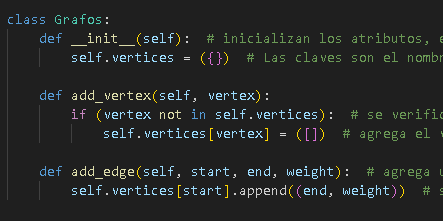
\includegraphics[width=0.8\textwidth]{figura_1_clase.PNG}
    \caption{Clase Grafos implementada en python}
    \label{figura 1}
\end{figure}
\begin{verbatim}
    __init__: El método __init__ se llama al crear un nuevo objeto de la 
    clase Graph. En este caso, inicializa el atributo vertices como un 
    diccionario vacío, donde las claves son los vértices y los valores son 
    listas de tuplas representando los vértices vecinos y los pesos de las 
    aristas.
    
    add_vertex: Este método agrega un vértice al grafo. Verifica si el 
    vértice ya está presente en el diccionario vertices antes de agregarlo.
    
    add_edge: Este método agrega una arista ponderada al grafo. Recibe el 
    vértice de inicio (start), el vértice final (end) y el peso de la arista 
    (weight). Añade una tupla (end, weight) a la lista de vecinos del vértice 
    de inicio en el diccionario vertices.
\end{verbatim}

Ahora, veamos la implementación de la función dijkstra:
\begin{figure}[H]
    \centering
    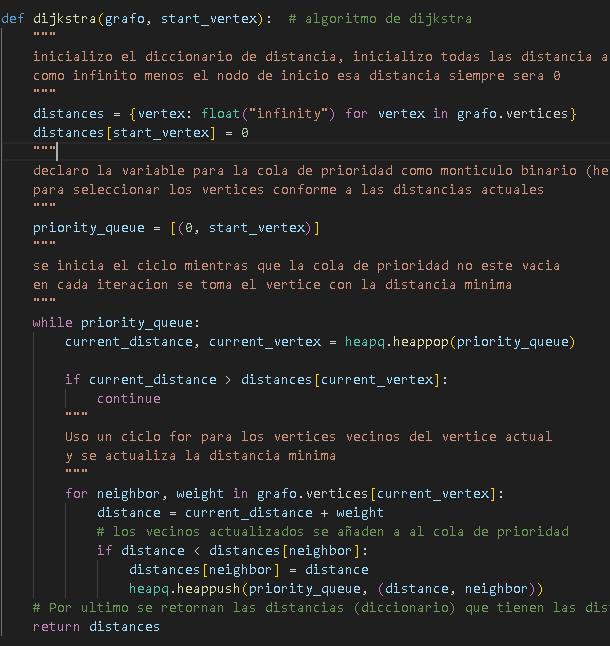
\includegraphics[width=0.8\textwidth]{figura_2_dijkstra.PNG}
    \caption{funcion de algoritmo de Dijkstra implementada en python}
    \label{figura 2}
\end{figure}
\begin{verbatim}
dijkstra: Esta función implementa el algoritmo de Dijkstra 
para encontrar los caminos mínimos desde un vértice de inicio 
hasta todos los demás vértices en un grafo ponderado dirigido.

Se inicializa un diccionario distances con distancias iniciales 
establecidas en infinito para todos los vértices excepto el vértice 
de inicio, que se establece en 0.

Se utiliza una cola de prioridad (priority_queue) implementada con 
un montículo binario para realizar selecciones eficientes de vértices 
basadas en sus distancias actuales.

El bucle principal se ejecuta mientras la cola de prioridad no esté vacía. 
En cada iteración, se extrae el vértice con la distancia mínima de la cola 
(heapq.heappop).

Se itera sobre los vecinos del vértice actual y se actualizan las distancias 
si se encuentra un camino más corto.

Los vecinos actualizados se añaden a la cola de prioridad (heapq.heappush).

El resultado final es un diccionario distances que contiene las distancias 
mínimas desde el vértice de inicio hasta todos los demás vértices.
\end{verbatim}

\begin{figure}[H]
    \centering
    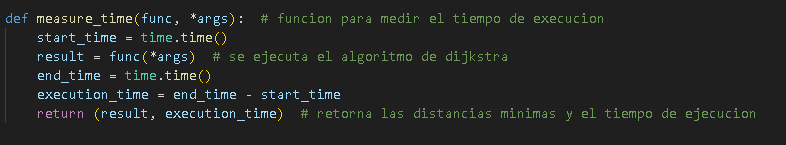
\includegraphics[width=0.8\textwidth]{figura_3_medicion_tiempo.PNG}
    \caption{funcion de medicion del tiempo implementada en python}
    \label{figura 3}
\end{figure}
\begin{verbatim}
    Finalmente, el código incluye una función measure_time para medir el 
    tiempo de ejecución.
\end{verbatim}
\subsection{Complejidad}
La complejidad temporal del algoritmo de Dijkstra con la implementación 
basada en una cola de prioridad mediante un montículo binario es de 
$O((V + E) \bullet log(V))$, donde V es el número de vértices y E es el número 
de aristas en el grafo.
\textbf{Análisis Manual:}
Inicialización:

Inicializar el diccionario distances con distancias iniciales: $O(V)$.
Inicializar la cola de prioridad $(priority_queue)$ con un vértice de inicio: 
$O(log(V))$.

Bucle Principal:

El bucle principal se ejecuta V veces (una vez por cada vértice).
En cada iteración del bucle:
Extraer el vértice con la distancia mínima de la cola de prioridad: $O(log(V))$.
Iterar sobre los vecinos del vértice actual: $O(E)$ en el peor caso.
Actualizar distancias y agregar vecinos a la cola de prioridad: $O(log(V))$ por 
cada vecino (en el peor caso).

Complejidad Final:

La complejidad del bucle principal es $O(V \bullet (log(V) + E \bullet log(V)))$.
La complejidad total es $O((V + E) \bullet log(V))$.
\section{Resultados y Conclusiones}
Caso 1:

\begin{figure}[H]
    \centering
    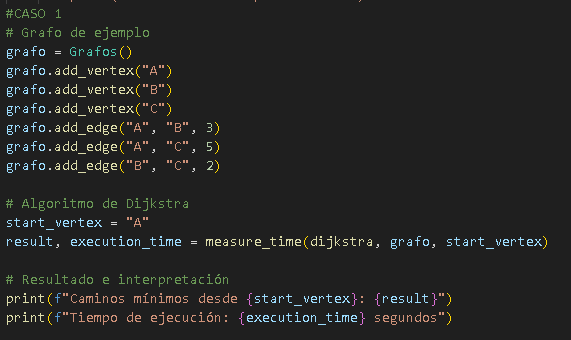
\includegraphics[width=0.8\textwidth]{figura_4_caso_1.PNG}
    \caption{Caso 1 de prueba}
    \label{figura 4}
\end{figure}
En este caso, el grafo es simple y no contiene ciclos negativos. 
El algoritmo de Dijkstra calculará las distancias mínimas desde el vértice 
de inicio "A" hasta todos los demás vértices. Se espera que los caminos 
mínimos sean "A" $\to$ "B" con distancia 3 y "A" $\to$ "C" con distancia 5.

Caso 2:

\begin{figure}[H]
    \centering
    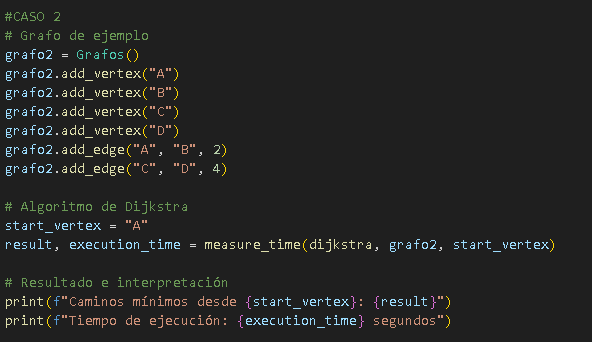
\includegraphics[width=0.8\textwidth]{figura_5_caso_2.PNG}
    \caption{Caso 2 de prueba}
    \label{figura 5}
\end{figure}
En este caso, el grafo está desconectado, lo que significa 
que no hay un camino entre algunos pares de vértices. El algoritmo de 
Dijkstra debe manejar correctamente esta situación y asignar distancias 
infinitas a los vértices inalcanzables desde el vértice de inicio "A".

Caso 3:

\begin{figure}[H]
    \centering
    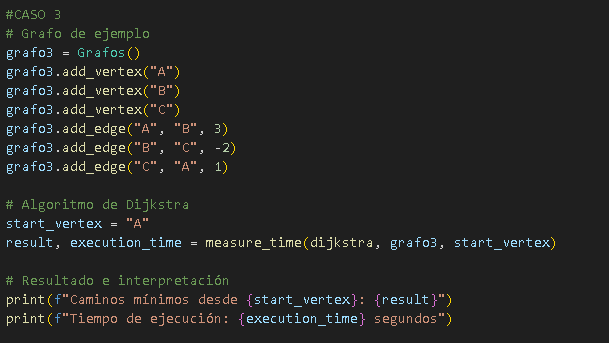
\includegraphics[width=0.8\textwidth]{figura_6_caso_3.PNG}
    \caption{Caso 3 de prueba}
    \label{figura 6}
\end{figure}
Este caso presenta un grafo que contiene un ciclo negativo. 
El algoritmo de Dijkstra no maneja adecuadamente ciclos negativos, 
ya que puede resultar en distancias mínimas incorrectas. En lugar de dar 
el camino mínimo, es probable que el algoritmo produzca resultados no válidos.

Caso 4:

\begin{figure}[H]
    \centering
    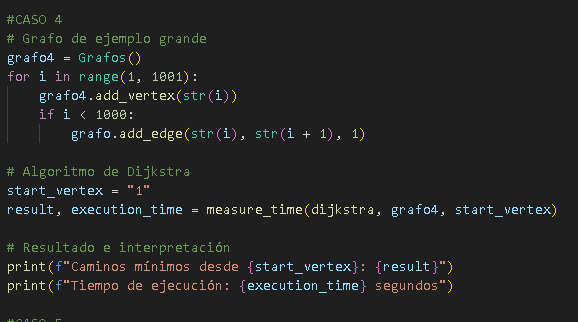
\includegraphics[width=0.8\textwidth]{figura_7_caso_4.PNG}
    \caption{Caso 4 de prueba}
    \label{figura 7}
\end{figure}
Este caso presenta un grafo grande con 1000 vértices 
conectados por aristas de peso 1. El algoritmo de Dijkstra debe manejar 
eficientemente grafos grandes sin ciclos negativos y calcular rápidamente 
las distancias mínimas.

Caso 5:

\begin{figure}[H]
    \centering
    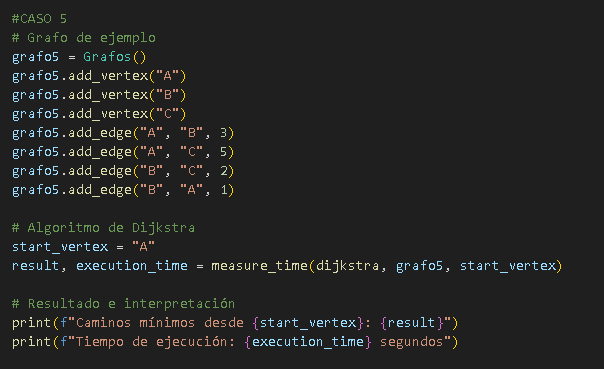
\includegraphics[width=0.8\textwidth]{figura_8_caso_5.PNG}
    \caption{Caso 5 de prueba}
    \label{figura 8}
\end{figure}
Explicación: Este caso presenta un grafo con aristas que tienen diferentes 
pesos en direcciones opuestas. El algoritmo de Dijkstra debe manejar 
correctamente este escenario y calcular las distancias mínimas de manera 
precisa. En este caso, se espera que el camino mínimo de "A" a "B" sea "A" $\to$ "B" con peso 1.

Resultados
\begin{figure}[H]
    \centering
    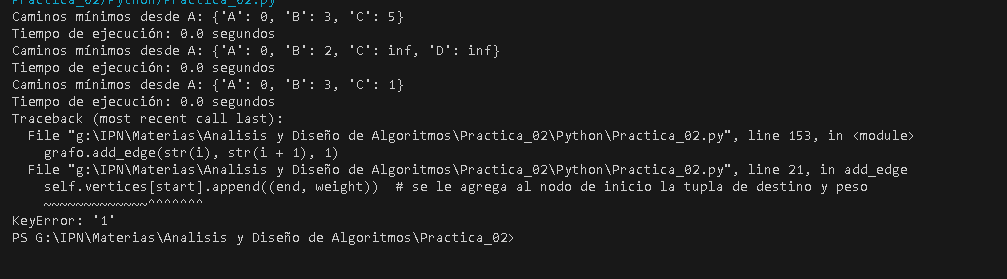
\includegraphics[width=0.8\textwidth]{resultados.PNG}
    \caption{Resultados}
    \label{figura 9}
\end{figure}

En conclusión, la implementación y exploración del algoritmo de Dijkstra 
han resultado exitosas en esta práctica. Hemos abordado el problema de 
caminos mínimos en grafos ponderados, destacando la importancia de este 
problema en la teoría de grafos y su relevancia en aplicaciones prácticas. 
La implementación en Python incluyó la definición de un grafo ponderado 
dirigido, la descripción detallada del algoritmo de Dijkstra y su aplicación 
en un caso de prueba específico.

Además, se llevó a cabo un análisis del algoritmo, incluyendo la medición del 
tiempo de ejecución para cada caso de prueba y el cálculo de su complejidad. 
Este análisis proporciona una comprensión profunda de la eficiencia del 
algoritmo en términos de tiempo y espacio, permitiendo evaluar su viabilidad 
en situaciones del mundo real. La práctica ha contribuido significativamente 
a la comprensión y aplicación de algoritmos clave en la resolución de 
problemas de optimización de rutas en diversos dominios.
\end{document}